% mechanism: a varwidth holding a display: the box's XML width is the measured width (VARWb) with `width:max-content;max-width:<given>`,
%   but the display's `ltx_eqn_table` (`display:block; max-width:100%` in `.ltx_inline-block`) and its padding cells push the
%   max-content size up to the max-width, so the HTML draws the box at its GIVEN width while `\resizebox`/TikZ read the measured one —
%   the equation lands over the next text. Fix: an `ltx_varwidth` marker + a CSS rule giving a display inside it its content's width,
%   or no `max-content` when the body holds a display (revVARWb S1; siblings: a wide `ltx_listing`, an `ltx_flex_figure`)
% witness: synthetic (revVARWb v5); none in VARWb's 21 changed A/B papers
% oracle:  pdflatex (TL 2025, -no-shell-escape) 0 `!`: `\wd` 39.46pt; "L [a+b=c scaled to 3cm] R"
% engines: rust VARWb: measured 39.46pt; Chrome draws the box 656px in a 114px outer box, over "R"; int164a fits it (113.8px)
% expect:  0 errors; the HTML box as wide as the display (the measured width)
% status:  RED (VARWb) — moves: post-merge (VWLD)
\documentclass{article}
\usepackage{varwidth,amsmath,graphicx,tikz}
\newsavebox\vb
\begin{document}
\sbox\vb{\begin{varwidth}{8cm}\[ a+b=c \]\end{varwidth}}\typeout{VW1=\the\wd\vb}
\sbox\vb{\begin{varwidth}{8cm}Short\begin{equation} E=mc^2 \end{equation}\end{varwidth}}\typeout{VW2=\the\wd\vb}

L \resizebox{3cm}{!}{\begin{varwidth}{8cm}\[ a+b=c \]\end{varwidth}} R

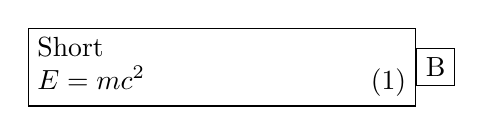
\begin{tikzpicture}
\node[draw] (A) {\begin{varwidth}{8cm}Short\begin{equation} E=mc^2 \end{equation}\end{varwidth}};
\node[draw,anchor=west] at (A.east) {B};
\end{tikzpicture}
\end{document}
